\section{Auswertung}
	\label{sec:auswertung}

	\subsection{Aufnahme der Charakteristik des Z"ahlrohrs} % (fold)
	\label{sub:z_ahlrohr_charakteristik}

	
\begin{table}[!h]
\begin{center}
\begin{tabular}{|r|r|r|r|r|r|}
\hline
U[$\SI{}{\volt}$] &	N & $\Delta$N & t[$\SI{}{\second}$] & N[$\SI{}{1\per\second}$] & $\Delta$N[$\SI{}{1\per\second}$]\\
\hline
\hline
300	 &   0	    & 0	&  140 & 0.00 & 0.00\\
310	 &   0	    & 0	&  140 & 0.00 & 0.00\\
315	 &   11849	& 108	&  140 & 84.64	& 0.77\\
320	 &   10374	& 101	&  120 & 86.45	& 0.84\\
325	 &   10302	& 101	&  120 & 85.85	& 0.84\\
330	 &   10216	& 101	&  120 & 85.13	& 0.84\\
340	 &   10596	& 103	&  120 & 88.30	& 0.86\\
360	 &   10611	& 103	&  120 & 88.43	& 0.86\\
380	 &   10697	& 103	&  120 & 89.14	& 0.86\\
430	 &   10840	& 104	&  120 & 90.33	& 0.87\\
480	 &   10725	& 104	&  120 & 89.38	& 0.87\\
530	 &   10784	& 104	&  120 & 89.87	& 0.87\\
560	 &   10924	& 105	&  120 & 91.03	& 0.88\\
580	 &   11039	& 105	&  120 & 91.99	& 0.88\\
600	 &   10734	& 104	&  120 & 89.45	& 0.87\\
620	 &   10853	& 104	&  120 & 90.44	& 0.87\\
640	 &   10788	& 104	&  120 & 89.90	& 0.87\\
690	 &   10961	& 105	&  120 & 91.34	& 0.88\\
700	 &   11032	& 105	&  120 & 91.93	& 0.88\\
705	 &   10917	& 104	&  120 & 90.98	& 0.87\\
710	 &   11073	& 105	&  120 & 92.28	& 0.88\\
715	 &   13063	& 114	&  120 & 108.86 &0.95\\
720	 &   12973	& 114	&  120 & 108.11 &0.95\\
\hline
\end{tabular}
\caption[Aufgabe a]{Messdaten zur Bestimmung der Charakteristik des Geiger-M"uller-Z"ahlrohrs.}
\label{tabellea}
\end{center}
\end{table}

	\begin{figure}[!h]
		\centering	
		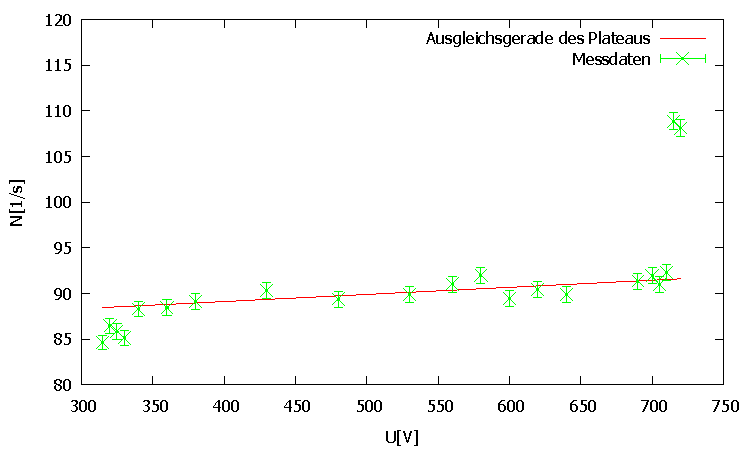
\includegraphics[width = 10cm]{img/charakteristik.pdf}
		\caption{Darstellung der Charakteristik des Z"ahlrohrs und einer Ausgleichsgeraden des Plateaus.}
		\label{charakteristik}
	\end{figure}

	Die Messungen f"ur die Charakteristik des Z"ahlrohrs ergaben die in Tabelle \ref{tabellea} aufgelisteten Werte. Eine graphische Darstellung findet sich in Graph \ref{charakteristik}.
	F"ur die Messung der Ausgleichsgeraden vom Typ $f(x) = m*x+b$ ergab sich:

	\begin{eqnarray*}
		m &=& \SI{0.00778 (169)}{1\per\volt\second}\\
		b &=& \SI{85.9993 (9144)}{1\per\second}
	\end{eqnarray*}

	Die Steigung der Geraden von $m = \SI{0.00778 (169)}{1\per\volt\second}$ entspricht einer Steigung von $\SI{0.99}{\%}$ pro $\SI{100}{\volt}$.
	Aus den Messdaten l"asst sich ablesen, dass die Plateaul"ange etwa $\SI{370}{\volt}$ betr"agt.
	Eine f"ur die Messung geeignete Z"ahlrohrspannung befindet sich am Anfang des Plateaus und liegt etwa bei $\SI{400}{\volt}$. Da sich dort der Arbeitsbereich des Geiger M"uller Z"ahlrohrs befindet sind die Anzahl der Nachentladungen noch gering.

	Die in der Tabelle errechneten Fehler der Impulsrate ergeben sich durch $\sqrt{N}$, da diese Poisson-Verteilt sind.

	\subsection{Sichtbarmachung von Nachentladungen und Messung der Totzeit mithilfe des Oszilloskops} % (fold)
	 \label{sub:sichtbarmachung_von_nachentladungen}

	\begin{table}[!h]
\begin{center}
\begin{tabular}{|r|r|}
\hline
$T_\mathrm{nach}$ & $\SI{200}{\micro\second}$ \\
$T_\mathrm{tot}$ & $\SI{200}{\micro\second}$
\hline
\end{tabular}
\caption[Aufbabe b,c]{Messdaten bei der Bestimmung der Nachentladungszeit $T_\mathrm{nach}$ und der Totzeit $T_\mathrm{tot}$ mithilfe des Oszilloskops.}
\label{tabelleb}
\end{center}
\end{table}
	
	F"ur die Bestimmung des zeitlichen Abstands zwischen Prim"ar- und Nachentladungsimpuls ergaben sich die in Tabelle \ref{tabelleb} aufgelisteten Werte. Daf"ur wurde die Zeit zwischen den auf dem Oszilloskop sichtbaren Maximas abgelesen.
	Da dies sehr ungenau ist, ist n"aherungsweise die Nachentladungszeit gleich der Totzeit.

	\subsection{Bestimmung der Totzeit mit der Zwei-Quellen-Methode} % (fold)
	\label{sub:bestimmung_der_totzeit_mit_der_zwei_quellen_methode}
	
	
\begin{table}[!h]
\begin{center}
\begin{tabular}{|l|r|r|r|r|r|}
\hline
Probe & N & $\Delta$N & t[$\SI{}{\second}$] & N[$\SI{}{1\per\second}$] & $\Delta$N[$\SI{}{1\per\second}$]\\
\hline
\hline
N1 & 13302	& 115 & 180 & 73.90 & 0.64 \\
N2 & 7902	& 89  & 360 & 21.95 & 0.27 \\
N12 & 16798	& 130 & 180 & 93.32 & 0.72 \\
\hline
\end{tabular}
\caption[Aufgabe d]{Messdaten zur Bestimmung der Totzeit $T_\mathrm{tot}$ mithilfe der Zwei-Quellen-Methode bei $\SI{450}{\volt}$.}
\label{tabelled}
\end{center}
\end{table}

	Bei der Messung ergaben sich die Werte aus Tabelle \ref{tabelled}.
	F"ur die Berechnung der Totzeit wurde die N"aherung \eqref{totzeit} verwendet.
	Es ergibt sich daraus:

	\begin{equation*}
		T_\mathrm{tot} = \SI{779.85 (29354)}{\micro\second} \quad .
	\end{equation*}

	Die Abweichung bez"uglich der Messung mit dem Oszilloskop k"onnte deshalb kommen, da wirklich nur sehr ungenau abgelesen werden konnte.
	Der Fehler Berechnet sich durch Gau"s'sche Fehlerfortpflanzung:

	\begin{eqnarray*}
		\frac{\partial T}{\partial N_\mathrm{1}} &=& \frac{2 N_\mathrm{1}N_\mathrm{2} - 2 N_\mathrm{2}(N_\mathrm{1} + N_\mathrm{2} - N_\mathrm{12})}{4N_\mathrm{1}^2N_\mathrm{2}^2} \, , \\
		\frac{\partial T}{\partial N_\mathrm{2}} &=& \frac{2 N_\mathrm{1}N_\mathrm{2} - 2 N_\mathrm{1}(N_\mathrm{1} + N_\mathrm{2} - N_\mathrm{12})}{4N_\mathrm{1}^2N_\mathrm{2}^2} \, ,\\
		\frac{\partial T}{\partial N_\mathrm{12}} &=& -\frac{1}{2 N_\mathrm{1} N_\mathrm{2}} \, ,\\
		\Delta T &=& \left( \left( |\frac{\partial T}{\partial N_\mathrm{1}}| \Delta N_\mathrm{1} \right)^2 + \left( |\frac{\partial T}{\partial N_\mathrm{2}}| \Delta N_\mathrm{2} \right)^2 + \left( |\frac{\partial T}{\partial N_\mathrm{12}}| \Delta N_\mathrm{12} \right)^2 \right)^\frac{1}{2} \quad .
	\end{eqnarray*}

	\subsection{Messung der pro Teilchen vom Z"ahlrohr freigesetzten Ladungsmenge} % (fold)
	\label{sub:messung_der_pro_teilchen_vom_z"ahlrohr_freigesetzten_ladungsmenge}
	
	
\begin{table}[!h]
\begin{center}
\begin{tabular}{|r|r|r|r|r|r|r|r|r|}
\hline
U[$\SI{}{\volt}$] N & $\Delta$ N & N[$\SI{}{1\per\second}$] & $\Delta$N[$\SI{}{1\per\second}$] & I[$\SI{}{\micro\ampere}$] & $\Delta$ I[$\SI{}{\micro\ampere}$] & Q \backslash Teilchen[$\SI{10 e10}{e}$] & $\Delta$ Q \backslash Teilchen[$\SI{10 e10}{e}$] \\
\hline
\hline
480	 &   10725 & 104 & 89.38  & 0.87 &	0.4	& 0.1 & 2.79 & 0.6998\\
580	 &   11039 & 105 & 91.99  & 0.88 &	0.5	& 0.1 & 5.44 & 0.6802\\
600	 &   10734 & 104 & 89.45  & 0.87 &	0.6	& 0.1 & 4.19 & 0.6992\\
620	 &   10853 & 104 & 90.44	& 0.87 &	0.6	& 0.1 & 4.14 & 0.6916\\
640	 &   10788 & 104 & 90.44	& 0.87 &	0.6	& 0.1 & 4.17 & 0.6957\\
\hline
\end{tabular}
\caption[Aufgabe e]{Messdaten}
\label{tabellee}
\end{center}
\end{table}

	\begin{figure}[!h]
		\centering
		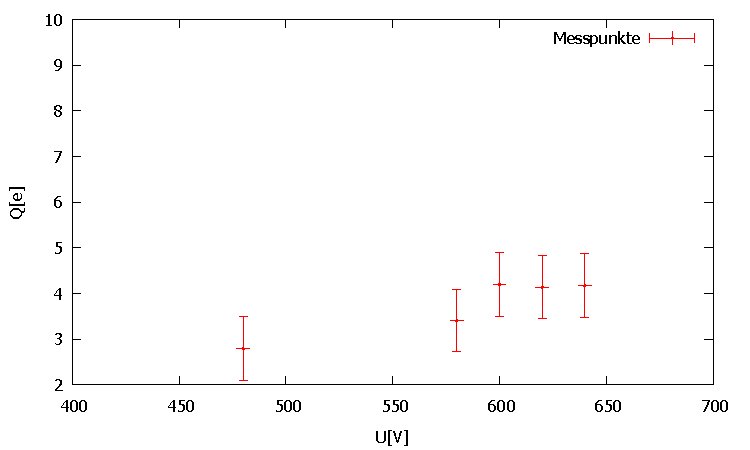
\includegraphics[width = 10cm]{img/ladung.pdf}
		\caption{Freigesetzte Ladung Q in Abh"angigkeit von der Spannung U}
		\label{ladung}
	\end{figure}

	Die Tabelle \ref{tabellee} zeigt die Ergebnisse zur Messung der pro Teilchen vom Z"ahlrohr freigestzten Ladungsmenge.
	Grafik \ref{ladung} zeigt die Freigesetzte Ladung Q in Abh"angigkeit von der Spannung U.